\chapter{Introduction to Organiztion}
\begin{figure}[ht]
	\centering
	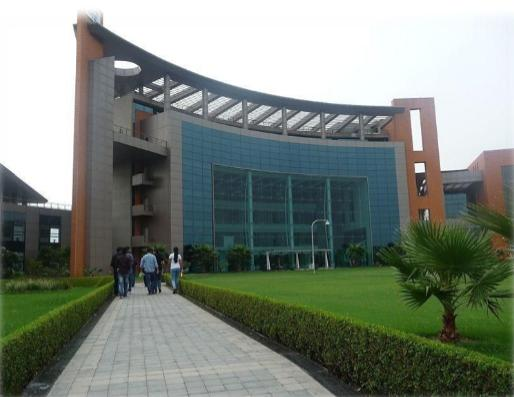
\includegraphics[width=3.5in, height=3in]{images/company.jpg}
	\caption{STMicroelectronics Pvt. Ltd., Greator Noida}
\end{figure}
\noindent STMicroelectronics is a world leader in providing the semiconductor solutions that make a positive contribution to people's lives, today and into the future.\\
\noindent Offering one of the industry's broadest product portfolios, ST serves customers across the spectrum of electronics applications with innovative semiconductor solutions for Smart Driving and the Internet of Things. %By getting more from technology to get more from life, ST stands for life.augmented.
\begin{itemize}
	\item Among the world's largest sermicondutor companies.
	\item A leading Integrated Device Manufacturer serving all electronics segments.
	\item A leading technology innovator (approximately 8,300 people working in R\&D, ~15,000 owned patents in ~9,000 patent families and 500 new patent filings).
	\item Delivering solutions that are key to Smart Driving and Internet of Things.
	\item Rich, balanced portfolio (ASICs, Application-Specific Standard Products and Multi-Segment Products).
	\item A pioneer and visionary leader in sustainibility.
	\item Corporate Headquarters: Geneva, Switzerland.
	\item President and CEO: Carlo Bozotti.
	\item 2015 revenue: \$6.90 billion.
	\item Approximately 43,200 employees.
	\item Over 75 sales \& marketing offices in 35 counteries.
	\item 11 main manufacturing sites.
	%\item Public ince 1994 - traded on New York Stock Exchange (NYSE: STM), Euronext Paris, and Borsa Italiana.
	\item Created as SGS-THOMPSON Microelectronics in June 1987, from merger of SGS Microelettronica (Italy) and Thomson Semiconducteurs (France).
	\item Renamed STMicroelectronics in May 1998.
\end{itemize}
